\chapter{Marco Teoríco}

En este capítulo veremos los principales conocimientos que son necesario para el entendimiento del presente seminario.
\section{GPGPU computing}
\subsection{CPU}(Central Processing Unit) es el hardware encargado del procesamiento de tareas mediante las operaciones básicas aritméticas, logicas y de entrada y salida del sistema. Los ordenadores actuales cuenta con más de una lo cual les permite usar multiprocesamiento. Los nucleos de la cpu estan hechos para el procesamiento de las tareas de manera secuencial.
Una CPU tiene 2 componentes principales:
+ **ALU (Unidad Aritmetica Logica):** se encarga de realizar las operaciones aritméticas y lógicas.
+ **CU  (Unidad de Control       ):** extrae información de la memoria la decodifica y ejecuta llamando a ALU las veces que sea necesario.

\subsection{GPU}
Las GPU(Graphics Processing Unit)
A diferencia de las CPU los GPU's estan compuestos de miles de nucleos que fueron diseñados para resolver tareas en paralelo.

\subsection{Procesamiento en Paralelo}
El procesamiento en paralelo consiste en dividir als instrucciones del programa en multiples procesadores con el objetivo de ejecutar el programa en menos tiempo.

\subsection{GPGPU} 
GPGPU(General Purpose Graphics Processing Unit) consiste en realizacción de los calculos que comumente serian realizados por el CPU utilizando GPU. Este método permite aprovechar los beneficios de potencia en procesamiento paralelos de las GPU's.
\begin{figure}[H]
	\centering
	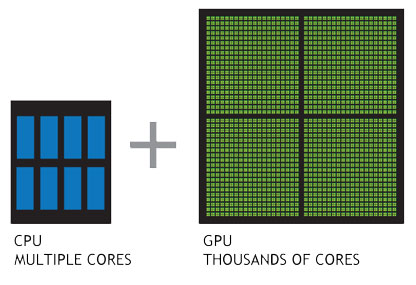
\includegraphics[width=0.9\textwidth]{Figures/cpu-and-gpu.jpg}
	\caption{Esquema GPGPU}
	\label{MVC}
\end{figure}



\section{Redes Neuronales}
\subsection{Neuronas}
En la biología la neurona es conocida como la unidad fundamental del cerebro humano, el cual está compuesto por millones de neuronas interconectadas entre si. El trabajo de las neuronas consiste en recibir información, procesarla y enviarla a otras células. Este modelo fue copiado en 1943 por Warren S. McCulloch y Walter H. Pitts. Analogamente con las neuronas del cerebro humano nuestra neuro artificial toma una cantidad n de entradas $x_{1}, x_{2}, x_{3}, .. , x_{n}$ estas entradas serán multiplicadas por pesos $w_{1}, w_{2}, w_{3}, .. , w_{n}$ además se puede añadir una constante que llamaremos bias. 

La entrada a de la neurona será la suma total de los productos z=  $\sum_{i=1}^{n}x_{i}$ , el valor de z será la entrada a la neurona la cual la evaluará con una función f de tal forma que nuestra salida sea $y=f(z)$. Otra forma de ver esta expresión es por medio de la notación de vectores donde representaremos a las entradas como $x= [x_{1}  x_{2}  x_{3}  ...  x_{n}]$ y los pesos w= $[w_{1}  w_{2}  w_{3}  ...  w_{n}]$ de esta manera la salida de la neurona estará dada por $y=f(x\cdot w+b)$ donde b representa las bias. 

\subsection{Redes Neuronales Artificiales}
Las redes neuronales artificiales(ANN)toman de ejemplo la arquitectura del cerebro como inspiración para la construcción de sistemas inteligente. Actualmente son la base para el desarrollo de la inteligencia artificial. Las redes neuronales están constituidas de las uniones de las neuronas.

\subsection{Redes Neuronales Profundas}


Las redes neuronales profundas estan constituidas principalmente de un numero de capas de convolución, No linearalidad y pooling.
\begin{itemize}
	\item Convolución:
	Un proceso importante dentro de las redes neuronales es la convolución que es usada para detectar las características de una imagen estas características pueden ser bordes, curvas, etc.
	\item No linearalidad:
	Debido a que las convoluciones son operaciones lineales, lo cual no es adecuado para las tareas del mundo real. Debido a esto es importante introducir el ReLu que aplicará funciones no lineales a los mapas de característica producidas en las capas de convolución.
	Una de las funciones las común es ReLu.
	\begin{figure}[H]
		\centering
		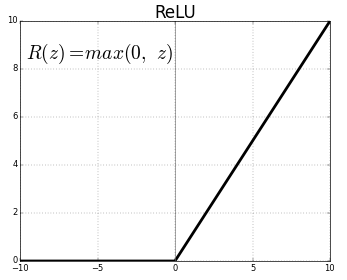
\includegraphics[width=0.5\textwidth]{Figures/relu.png}
		\caption{ReLu}
		\label{ReLu}
	\end{figure}

	
	\item Pooling:
	Sirve para transformar el mapa de características en una representación de menor dimensión con el objetivo de la red sea más invariante a pequeñas transformaciones o variación de la imagen de entrada.
\end{itemize}

\section{Herramientas}
\subsection{TensorFlow}
Es un framework open source de google que nos permite realizar multiples técnicas de deep learning. TensorFlow nos provee de multiples API's en el nivel bajo de la API nos provee completo control en la programación y el nivel más alto nops permite que las tareas repetitivas sean más faciles y consistente.
Además la arquitectura flexible nos permite implementar cálculos a una a o más CPU's o GPUs, actualmente este framework es usado por muchas compañias como inte, Nvidia,UBER, etc.
	\begin{figure}[H]
		\centering
		
\includegraphics[width=0.5\textwidth]{Figures/tensorflow}
		\caption{TensorFlow}
		\label{TensorFlow}
	\end{figure}

%%\subsubsection*{Características}
%%%
%%\begin{figure}[H]
%%\centering
%%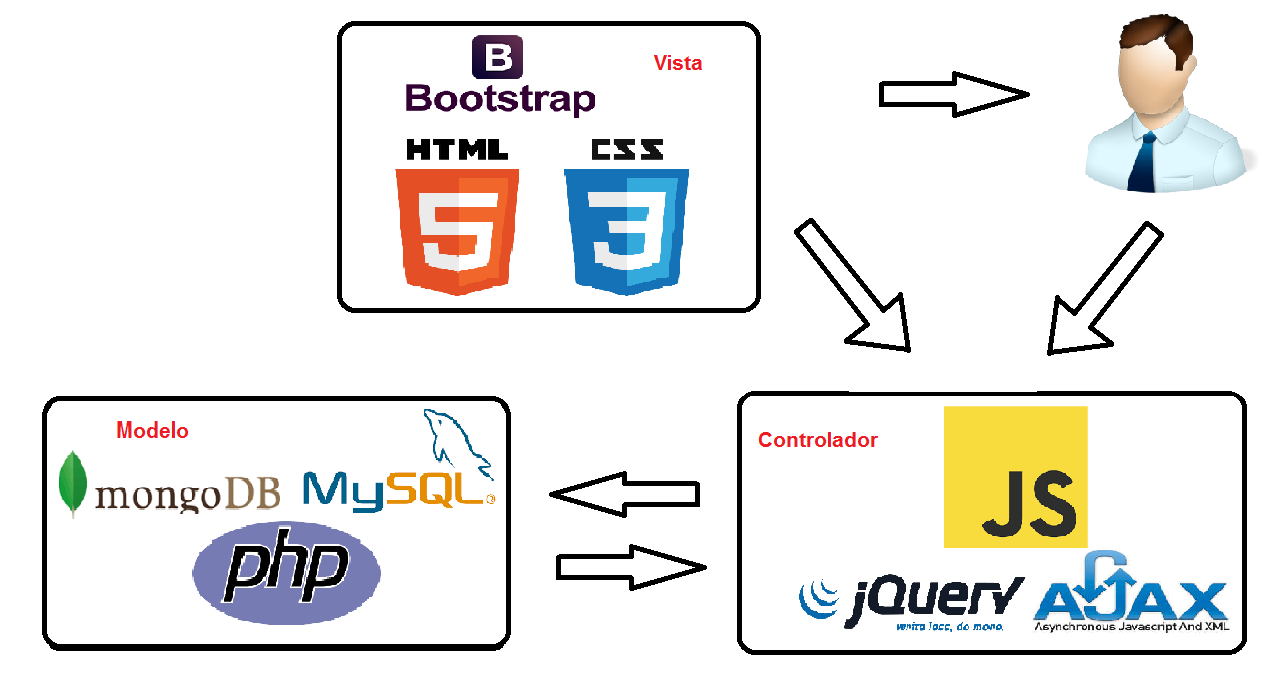
\includegraphics[width=0.9\textwidth]{Figures/mvc.png}
%%\caption{Modelo-Vista-Conrolador}
%%\label{MVC}
%%\end{figure}



\afterpage{\blankpage}